\subsubsection{Grazing}

\begin{prop}
  $f$ tiene un punto m\'aximo en $\mathbb{R}^+$ si y solo s\'i $\phi > (D_i - 1)p_d$ 
\end{prop}

\begin{proof}
\mbox{}\\
Sea $ h = (D_i-1)p_d$\\
Dado que $f$ es diferenciable y:
  \begin{equation}
    \begin{aligned}
      f'(k_{ij}) &= a \frac{h k_{ij}^{h-1} (1 + k_{ij}^\phi) -\phi k_{ij}^{\phi-1+h}}{(1+k_{ij}^{\phi})^2} \\
            &= a \frac{(h-\phi)k_{ij}^{h-1 + \phi}  + h k_{ij}^{h-1} }{(1+k_{ij}^{\phi})^2}\\
            &= a \frac{(h-\phi)k_{ij}^\phi + h }{(1+k_{ij}^{\phi})^2}\\
     \end{aligned}
  \end{equation}
Luego tenemos que $f'$ posee un \emph{cero} en $\mathbb{R}^+$ si y solo s\'i $ h< \phi$ y en caso afirmativo tenemos que $k^*$ tal que $f(k^*) = 0$ es $(\frac{h}{\phi-h})^{\frac{1}{\phi}}$ adem\'as:
\begin{equation}
  f'(x) :
  \begin{cases}
    < 0 &; k_{ij}  > k^* \\
    > 0 &; k_{ji} < k^*
  \end{cases}
\end{equation}

Lo que indica que $k^*$ es un punto m\'aximo.
\end{proof}

De la proposici\'on anterior tambi\'en vemos la dependencia de $k^*$ en $\phi$, teniendo $h$ fijo en nuestro caso se observa que si $\phi$ esta suficientemente cercano a $h$ , $k^*$ es extremadamente grande, sin embargo se observa un decaim\'iento muy r\'apido y para valores de $\phi \geq 2h$  , $k^*$ se encuentra pr\'oximo a 1(y en realidad converge a 1 para $\phi \to \infty$) , v\'ease figura \ref{fig:kmaxGrazing}. \\

\begin{figure}
\begin{center}
 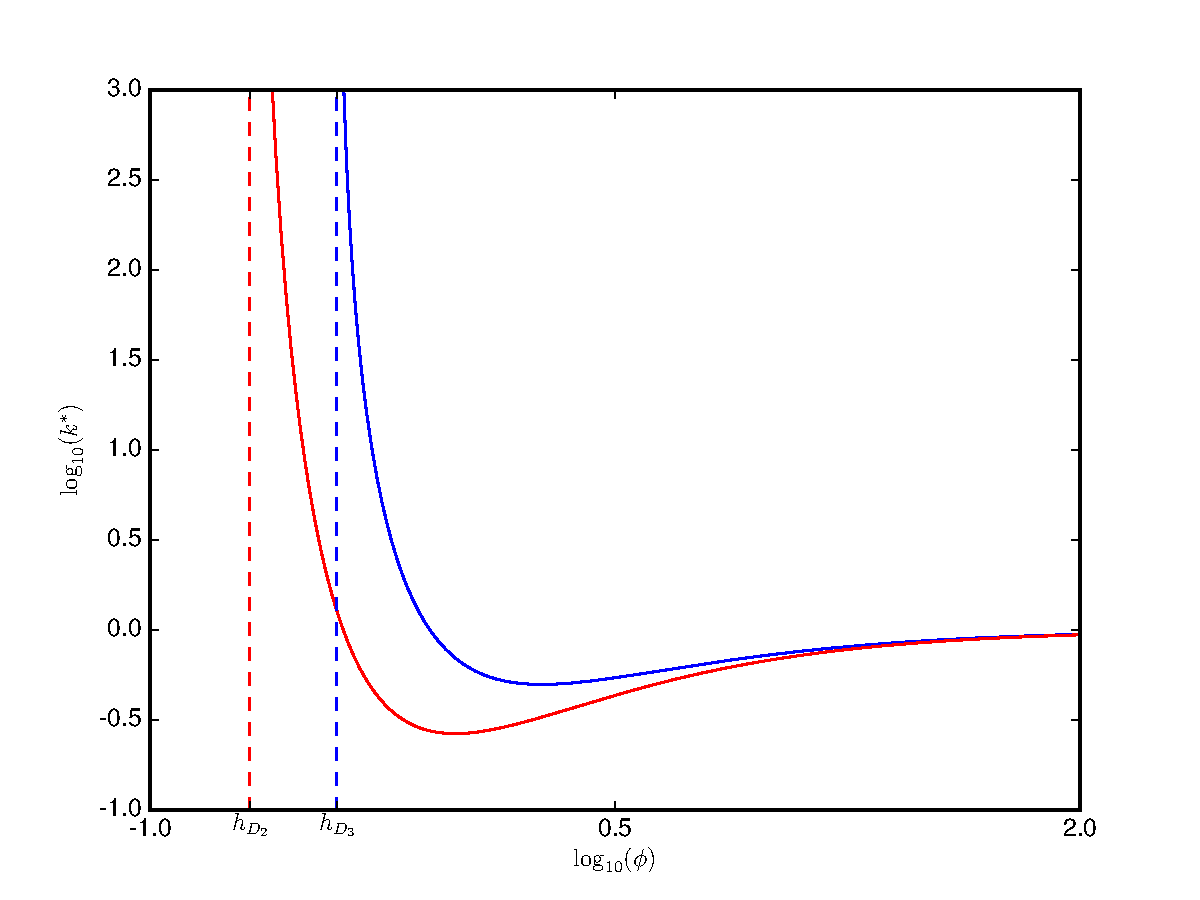
\includegraphics[width=0.9\textwidth]{./Plots/kmaxGrazing.pdf}
 \caption[$k^*, Grazing$]{$k^*$ en funci\'on a $\phi$ donde se observa la divergencia para valores cercanos a $h$ y la convergencia a 1 para valores elevados de $\phi$, ({\hwplotB}) es para el caso de ambientes de b\'usqueda $3D$ y ({\hwplotR}) $2D$, $h_{3D}$ y $h_{2D}$ denotan los l\'imites inferiores para $\phi$ que permiten la existencia de $k^*$}
 \label{fig:kmaxGrazing} 
\end{center}
\end{figure}


A su vez tenemos que en el caso $ \phi > h$ :
\begin{equation}
  \lim_{k_{ij} \to \infty} f(k_{ij}) - k_{ij}^{h - \phi} = 0
\end{equation}

Por lo tanto $ f \approx k_{ij}^{h - \phi}$ para valores de $k_{ij}$ \emph{suficientemente grandes}. En el caso que $\phi < h$ tenemos que $f$ es mon\'otona creciente. Ambos casos se grafican en la figura \ref{fig:f1Grazing}.

\begin{figure}
\begin{center}
 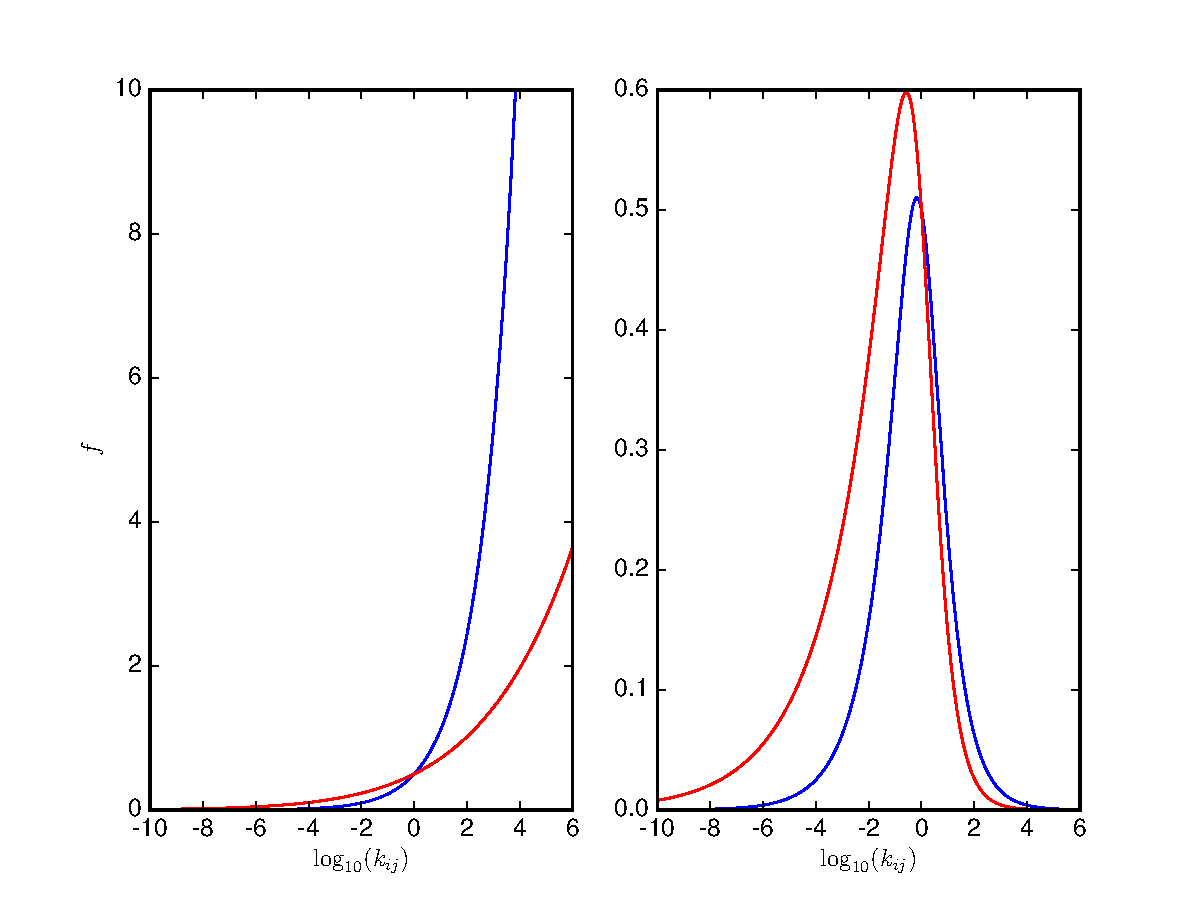
\includegraphics[width=0.9\textwidth]{./Plots/f1Grazing.pdf}
 \caption[$f_1, Grazing$]{$f$ en funci\'on a $k_{ij}$, con $a =1$, en el panel de la izquierda tenemos $b = 0.1$ y en el de la derecha $b=1.$ , ({\hwplotB}) es para el caso de ambientes de b\'usqueda $3D$ y ({\hwplotR}) $2D$, en ambos casos se observa que $f \approx k_{ij}^{h}$ para valores de $k_{ij}$ peque\~nos y en el panel derecho que $f \approx k_{ij}^{h - \phi}$ para $k_{ij}$ suficientemente grande.}
 \label{fig:f1Grazing} 
\end{center}
\end{figure}

